\selectlanguage{english}
\clearpage
\section{Tool Evaluation and Selection}

This chapter presents an evaluation of available tools and test frameworks that could be used to support the integration testing of IPC middleware. The goal is to identify solutions that align with the defined testing requirements and environmental constraints presented in the previous chapter. Based on a set of defined selection criteria, several tool candidates are reviewed and assessed in terms of their compatibility with eCAL and the specific demands of testing distributed communication systems.

\subsection{eCAL as a Middleware Solution for IPC Testing}

\textbf{Overview and Architecture}

\vspace{0.4em}
eCAL (enhanced Communication Abstraction Layer) is a flexible middleware designed for efficient inter-process communication (IPC). It supports various transport layers, such as shared memory for communication on a single machine, and UDP or TCP for communication over a network. eCAL automatically selects the most suitable transport method based on system conditions \cite{ecal_official_docs}.


\vspace{1em}
\begin{figure}[H]
	\centering
	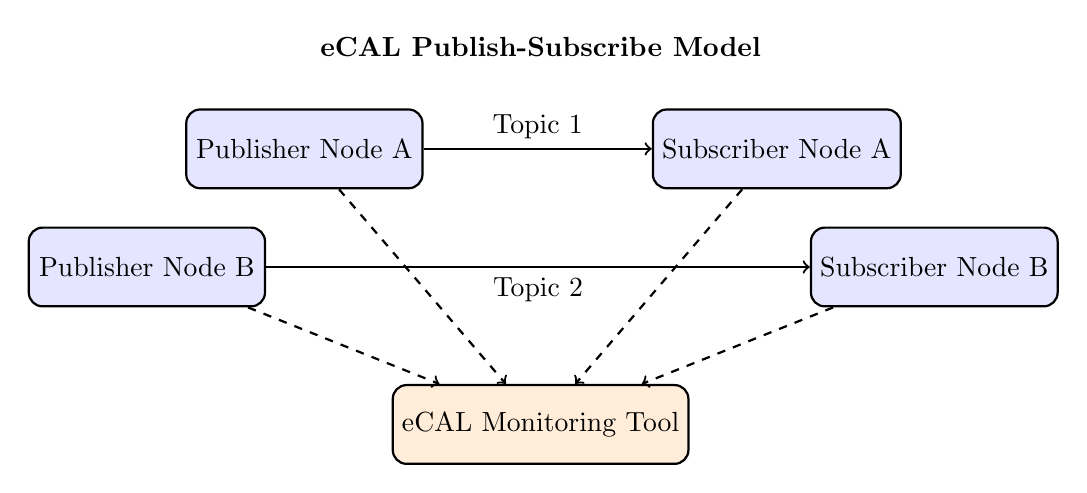
\begin{tikzpicture}[
		component/.style={draw, thick, minimum width=3cm, minimum height=1cm, rounded corners=5pt, fill=blue!10},
		arrow/.style={->, thick}
		]
		
		\node[component] (pub1) at (0,2.5) {Publisher Node A};
		\node[component] (pub2) at (-2,1) {Publisher Node B};
		\node[component] (sub1) at (6,2.5) {Subscriber Node A};
		\node[component] (sub2) at (8,1) {Subscriber Node B};
		\node[component, fill=orange!15] (monitor) at (3,-1) {eCAL Monitoring Tool};
		
		\draw[arrow] (pub1) -- node[above] {Topic 1} (sub1);
		\draw[arrow] (pub2) -- node[below] {Topic 2} (sub2);
		\draw[arrow, dashed] (pub1) -- (monitor);
		\draw[arrow, dashed] (pub2) -- (monitor);
		\draw[arrow, dashed] (sub1) -- (monitor);
		\draw[arrow, dashed] (sub2) -- (monitor);
		
		\node at (3,3.8) {\textbf{eCAL Publish-Subscribe Model}};
	\end{tikzpicture}
	\caption{Simplified architecture of the eCAL framework with publisher, subscriber, and monitoring components}
	\label{fig:ecal_architecture}
\end{figure}

\newpage
Figure~\ref{fig:ecal_architecture} shows the basic structure of the eCAL system. It includes publisher and subscriber nodes that exchange messages over topics. A built-in monitoring tool observes the communication to support debugging and system analysis.

\vspace{1.2em}
\textbf{Main Features}

\vspace{0.4em}
eCAL offers several features that are useful for real-time and distributed systems:

\begin{itemize}
	\item \textbf{High Performance:} Thanks to zero-copy in shared memory mode, eCAL can transmit data with very low latency and high throughput~\cite{ecal_github,ecal_official_docs}.
	
	\item \textbf{Multi-Language Support:} It provides APIs for C++, C\#, Python, Java, and Go, which makes it easy to use in different projects~\cite{ecal_official_docs}.
	
	\item \textbf{Cross-Platform Support:} eCAL works on Windows, Linux, and macOS, making it suitable for many system environments~\cite{ecal_official_docs}.
	
	\item \textbf{Integrated Tools:} eCAL includes tools for monitoring, recording, replaying, and analyzing communication, which are helpful during development and testing~\cite{ecal_github,ecal_official_docs}.
\end{itemize}

\vspace{1.2em}
\textbf{Benefits and Challenges}

\vspace{0.4em}
Middleware like eCAL helps to manage communication between software modules in a structured way. It reduces the need to handle low-level networking code and allows systems to scale more easily. On the other hand, middleware adds complexity and can make debugging and performance tuning more difficult. Especially in real-time systems, the overhead from abstraction can become a limitation.

\vspace{1em}
\textbf{Limitations of Current Testing Approaches}

\vspace{0.4em}
Although eCAL includes helpful tools for monitoring and debugging, it does not provide a complete solution for full system testing. Most available tools are designed for developers and focus on individual components rather than entire communication workflows. To test distributed behavior, such as message loss over UDP, transmission delays over TCP, or network interruptions, additional tools and setups are required. In practice, this often means running publishers and subscribers in isolated Docker containers to simulate real network conditions. Without containerization, it is difficult to create realistic and repeatable test environments for distributed communication.


\subsection{Test Tool Selection Criteria}

To choose suitable testing tools and frameworks, several criteria were defined:

\begin{itemize}
	\item \textbf{Command Line Interface (for Automation):} The tool should support execution via command line to allow headless automation and scripting in CI/CD environments.
	\item \textbf{Multi-Process Orchestration:} The tool should be able to handle the orchestration of multi-process communication patterns, such as publish-subscribe and request-response.
	\item \textbf{Open Source Availability:} Preference is given to open-source tools to ensure transparency, adaptability, and long-term maintainability.
	\item \textbf{CI/CD - Automation Capabilities:} Support for test automation, headless execution, and integration into CI/CD systems is essential.
	\item \textbf{Platform Compatibility:} The framework must work on Linux and Windows, as these is the primary target platform.
	\item \textbf{Observability and Reporting:} Tools should offer logging, result exporting, or structured test result visualization (e.g., HTML reports).

\end{itemize}

\subsection{Evaluation of Tool Candidates}

\subsubsection*{GoogleTest}

GoogleTest is a widely used testing framework for C++ applications. It provides many useful macros and assertions that help developers write automated tests for individual functions, classes, and modules. In the eCAL project, GoogleTest is already used to verify internal logic, data handling, and utility functions. This makes it a good choice for unit testing, especially during early development stages.

\vspace{1em}
However, GoogleTest is mainly designed for unit testing and does not support tests that involve multiple running processes. Integration testing of IPC middleware usually requires testing communication between different processes such as publishers and subscribers. To use GoogleTest in this context, additional scripts or wrapper functions are needed to start processes and simulate communication. While this is possible, it increases the complexity of test setups and reduces maintainability. Therefore, GoogleTest should be combined with other tools when performing full integration tests. More information is available in the official GoogleTest documentation~\cite{GoogleTestDocs}.

\subsubsection*{Robot Framework}

Robot Framework is a general-purpose, open-source test automation framework. It follows a keyword-driven approach, allowing users to write tests in a readable and structured way. Tests are usually written in plain text and can be run through the command line or integrated into automated systems.

\vspace{1em}
One of the key strengths of Robot Framework is its flexibility and support for integration testing. With built-in libraries such as \texttt{Process}, \texttt{OperatingSystem}, and \texttt{BuiltIn}, it can start and stop applications, check logs, and validate output. These features are especially helpful for testing IPC middleware like eCAL, where several processes must run in parallel and communicate correctly. For example, Robot Framework can launch both publishers and subscribers, wait for data exchange, and verify the results.

\vspace{1em}
Another important feature is automatic report generation. After each test run, Robot Framework produces HTML and XML reports that show test results, timing, and logs. This is very useful for continuous integration pipelines that run tests regularly. The official Robot Framework User Guide provides further details~\cite{RobotFrameworkDocs}.

\subsubsection*{Gauge Test}

Gauge is a modern test framework developed by ThoughtWorks. It lets users write test scenarios in Markdown format, which helps make tests easier to read and maintain. These scenarios are then connected to test code written in programming languages like Java, Python, or C\#. Gauge also supports running tests in parallel and generating HTML reports.

\vspace{1em}
Although Gauge has many useful features, it is mostly used for testing web applications, APIs, and user interfaces. It is not specifically designed for backend systems like IPC middleware. Also, its community is relatively small, and there are fewer plugins available compared to larger frameworks.

\vspace{1em}
Using Gauge for testing IPC would require custom scripts and additional effort to manage process orchestration. Because of this, Gauge is not the best fit for testing systems like eCAL. Further documentation can be found on the official Gauge website~\cite{GaugeDocs}.

\newpage
\subsubsection*{Katalon and TestComplete}

 Katalon and TestComplete are test tools mainly used for testing web interfaces, APIs, and desktop applications. They often include graphical interfaces for designing and running tests, and they support features like recording user actions and parameterizing input values.

\vspace{1em}
However, these tools are not intended for testing IPC systems. They do not support low-level message handling or process orchestration, which are important when testing middleware like eCAL. In addition, most of these tools are not open source, and they often rely on graphical interfaces, which makes them less suitable for headless environments or automation using Docker and CLI.

\vspace{1em}
For these reasons, these tools are not recommended for integration testing of eCAL or similar IPC frameworks. More information can be found in their official documentation~\cite{KatalonDocs,TestCompleteDocs}.

\subsubsection*{behave and Behavior-Driven Development (BDD)}

Another approach worth mentioning is Behavior-Driven Development (BDD), which combines principles from test-driven development (TDD) and domain-driven design (DDD). BDD focuses on describing software behavior in a language that both developers and non-developers can understand~\cite{North2006}.

\vspace{1em}
A popular Python framework for BDD is \texttt{behave}~\cite{BehaveDocs}, which uses the Gherkin syntax (Given–When–Then) to define executable specifications. The actual test logic is implemented in Python, offering flexibility for system and integration testing scenarios. However, orchestration and reporting must be implemented separately using custom Python scripts or shell tools.

\newpage
\subsection{Tool Selection for Middleware Testing}

\vspace{0em}
Table~\ref{tab:framework_comparison_reporting} presents an overview of evaluated tools in this Chapter.

\begin{table}[H]
	\centering
	\renewcommand{\arraystretch}{1.4}
	\begin{tabular}{|p{2.8cm}|p{1cm}|p{1.8cm}|p{1.2cm}|p{1cm}|p{1cm}|p{1.8cm}|}
		\hline
		\textbf{Framework} & \textbf{CLI} & \textbf{Multi- Process} & \textbf{Open- Src} & \textbf{CI/ CD} & \textbf{Plat- form} & \textbf{Reports} \\
		\hline
		\textbf{Google Test}         & \cmark & Partial & \cmark & \cmark & \cmark & XML only \\
		\hline
		\textbf{Robot Framework}     & \cmark & Yes     & \cmark & \cmark & \cmark & HTML, XML \\
		\hline
		\textbf{Gauge Test}          & \cmark & Limited & \cmark & \cmark & \cmark & HTML \\
		\hline
		\textbf{behave (BDD)}        & \cmark & Partial & \cmark & \cmark & \cmark & Text/ Custom \\
		\hline
		\textbf{Katalon}             & \xmark & No      & \xmark & \xmark & \cmark    & HTML, GUI \\
		\hline
		\textbf{TestComplete}        & \xmark & No      & \xmark & \xmark & \cmark   & HTML, GUI \\
		\hline
	\end{tabular}
	\caption{Comparison of test frameworks for IPC middleware testing with focus on multi-process orchestration}
	\label{tab:framework_comparison_reporting}
\end{table}


Following the evaluation of multiple testing frameworks, Robot Framework was identified as a suitable tool for integration testing in middleware-based systems. It fulfills key requirements such as support for keyword-driven test definitions, automation of command-line tools, and coordination of multiple parallel processes. These features are valuable when testing communication patterns like publish-subscribe or service-based exchanges.

\vspace{1em}
An alternative to Robot Framework is \texttt{behave}, which is suitable for teams following a BDD approach. It enables human-readable scenario definitions and flexible test logic using Python. However, since \texttt{behave} lacks built-in features for process orchestration and structured reporting, it requires additional scripting and infrastructure to reach the same level of automation. For the use case of testing IPC middleware like eCAL, where containerized process management and test reproducibility are critical, Robot Framework remains the more practical and efficient choice.

\vspace{2em}
For unit-level testing of individual components, GoogleTest remains the preferred choice. Its compatibility with C++ and strong support for isolated module testing make it a practical solution for verifying internal logic, data processing, and error handling at the code level. By combining Robot Framework for system-level validation with GoogleTest for component-level checks, a comprehensive and layered testing strategy can be achieved.

\subsection{Summary}

This chapter presented a comparative evaluation of tools and frameworks suitable for testing IPC middleware systems. After outlining the architecture and current testing limitations of the eCAL framework, a set of tool selection criteria was defined to guide the evaluation process. Multiple frameworks were assessed, including GoogleTest, Robot Framework, Gauge, behave, Katalon, and TestComplete.

\vspace{0.5em}
The results show that while GoogleTest is well-suited for unit testing of C++ components, it lacks support for orchestrating multi-process communication. On the other hand, Robot Framework offers strong capabilities for integration testing, including process control, CLI automation, and report generation, making it a practical choice for testing middleware. Gauge and behave offer readable test syntax but require additional scripting for IPC use cases. GUI-based tools like Katalon and TestComplete are not suitable for headless, distributed middleware testing.

